
%(BEGIN_QUESTION)
% Copyright 2012, Tony R. Kuphaldt, released under the Creative Commons Attribution License (v 1.0)
% This means you may do almost anything with this work of mine, so long as you give me proper credit

This temperature control system has a problem.  The customer complains that ``there is no hot air coming out of the collector'' and that the system needs to be fixed {\it now}.  The output display on the controller registers 102.5\%:

$$\includegraphics[width=15.5cm]{i01109x01.eps}$$

A fellow technician suggests to put the controller into manual mode, to get the system working again at least until a proper diagnosis can be made as to why there is no hot air coming out of the collector.  When you arrive on the scene, you measure 120 volts AC to the ``power'' teminals on the variable-speed motor drive and 5.1 volts DC to the ``input'' terminals on the motor drive.

\vskip 10pt

First, identify whether or not you would follow your fellow technician's suggestion to place the controller in manual mode, based on what you know about the system so far.  If so, explain why.  If not, explain why not.

\vskip 50pt

Next, identify the next diagnostic test you would perform, and the rationale for performing that test.

\underbar{file i01109}
%(END_QUESTION)





%(BEGIN_ANSWER)

5 points for assessing suggestion with explanation, 5 points for next test with explanation.  Deduct 3 points per wrong or missing explanation.

\vskip 10pt

The suggestion to put the controller in manual is pointless, because we already know the motor drive is receiving a 95\% signal, which ought to be enough to drive the fan fast.  The fan isn't pushing air, so the problem is not in the controller and won't be rectified by switching to manual.

\vskip 10pt

If there is no air coming out of the collector, the most logical next test to do is to measure DC voltage going to the fan motor: this will tell you if the motor drive circuit is doing its job or not.  At this point, we have reason to believe the over-setpoint temperature measurement is correct, and that the controller is doing its job.  The problem must lie either with the motor or with the motor drive.

\vskip 10pt

Another possibility is that the customer's complaint about there being ``no hot air'' might mean there's plenty of airflow, just cold and not hot.  Given this interpretation, perhaps the problem is a fan running at full speed because the controller ``thinks'' it's reading a high collector temperature.  In this case the most logical next test would be to verify the temperature reading (perhaps measure thermocouple voltage or the PV milliamp signal to the controller).

%(END_ANSWER)





%(BEGIN_NOTES)

{\bf This question is intended for exams only and not worksheets!}.

%(END_NOTES)


